
% Include LaTeX packages
\documentclass[conference]{styles/acmsiggraph}
\usepackage{comment} % enables the use of multi-line comments (\ifx \fi)
\usepackage{fullpage}
\usepackage{enumitem}
\usepackage{amsmath,amsthm,amssymb}
\usepackage{listings}
\usepackage{graphicx}
\usepackage{etoolbox}
\usepackage{verbatim}
\usepackage[dvipsnames]{xcolor}
\usepackage{fancyvrb}
\usepackage{hyperref}
\usepackage{menukeys}
\usepackage{titlesec}
\usepackage{csquotes}
\usepackage{placeins}
\usepackage{algorithm} 
\usepackage{algpseudocode}
\usepackage{unicode-math}
\newcommand{\?}{\stackrel{?}{=}}

% Set additional LaTeX options
\setlength{\parskip}{.8mm}
\setcounter{MaxMatrixCols}{20}
\hypersetup{
	colorlinks=true,
	urlcolor=[rgb]{0.97,0,0.30},
	anchorcolor={0.97,0,0.30},
	linkcolor=black,
	filecolor=[rgb]{0.97,0,0.30},
}

% Define title, author, and affiliation information
\title{\huge PSET 2 \\ \LARGE {CS124: Data Structures and Algorithms \\ Prof. Mitzenmacher}}
\author{\Large Dhilan Ramaprasad \\ dhilanramaprasad@college.harvard.edu}
\pdfauthor{Student Name}

% Redefine \VerbatimInput
\RecustomVerbatimCommand{\VerbatimInput}{VerbatimInput}%
{fontsize=\footnotesize,
 %
 frame=lines, % top and bottom rule only
 framesep=2em, % separation between frame and text
 rulecolor=\color{Gray},
 %
 label=\fbox{\color{Black}\textbf{OUTPUT}},
 labelposition=topline,
 %
 commandchars=\|\(\), % escape character and argument delimiters for commands within the verbatim
 commentchar=* % comment character
}

% Set addditional formatting options
\titlespacing*{\section}{0pt}{5.5ex plus 1ex minus .2ex}{2ex}
\titlespacing*{\subsection}{0pt}{3ex}{2ex}
\setcounter{secnumdepth}{4}
\renewcommand\theparagraph{\thesubsubsection.\arabic{paragraph}}
\newcommand\subsubsubsection{\paragraph}

% Define a convenient norm symbol
\newcommand{\norm}[1]{\left\lVert#1\right\rVert}
\renewcommand{\vec}[1]{\mathbf{#1}}

% Define a macro for hiding answers
\newbool{hideanswers} \setbool{hideanswers}{false}
\newenvironment{answer}{}{}
\ifbool{hideanswers}{\AtBeginEnvironment{answer}{\comment} %
\AtEndEnvironment{answer}{\endcomment}}{}

% Define text formatting for points and normals
\newcommand{\points}[1]{\hfill \normalfont{(\textit{#1pts})}}
\newcommand{\pointsin}[1]{\normalfont{(\textit{#1pts})}}







%%%%%%%%%%%%%%%%%%%%%%%%%%%%%%%%%%%%%%%
%%%%%%%%%%%%%%%%%%%%%%%%%%%%%%%%%%%%%%%
%%%%%%%%%%%%%%%%%%%%%%%%%%%%%%%%%%%%%%%
%%%%%%%%%%%%%%%%%%%%%%%%%%%%%%%%%%%%%%%
%%%%%%%%%%%%%%%%%%%%%%%%%%%%%%%%%%%%%%%

         %  START HERE  %

%%%%%%%%%%%%%%%%%%%%%%%%%%%%%%%%%%%%%%%
%%%%%%%%%%%%%%%%%%%%%%%%%%%%%%%%%%%%%%%
%%%%%%%%%%%%%%%%%%%%%%%%%%%%%%%%%%%%%%%
%%%%%%%%%%%%%%%%%%%%%%%%%%%%%%%%%%%%%%%
%%%%%%%%%%%%%%%%%%%%%%%%%%%%%%%%%%%%%%%

\begin{document}
\maketitle

Preface if needed here.


%%%%%%%%%%%%%%%%%%
%   Question #1  %
%%%%%%%%%%%%%%%%%%
\section{StoogeSort} \label{number1}

\subsection{Algorithm Explanation}
Before we dive into a proof of correctness, it is important to further qualify details of the algorithm as described in the homework description.  

\subsubsection{What is two-thirds?} \label{two-thirds}
Let's first take the sorting algorithm as given: sort first two-thirds, then the last two-thirds, then the first two-thirds, again.  (We'll consider the recursion aspect later.)  Here's an example list (whose number of elements is not divisible by three):
$$\{54, 38, 232, 15, 3, 8, 10\}$$
Sorting the first two-thirds (but assuming that two-thirds of the seven-element list rounds down to 4-elements):
$$\{15, 38, 54, 232, 3, 8, 10\}$$
Sorting the last two-thirds (again assuming that two-thirds of the seven-element list rounds down to 4-elements):
$$\{15, 38, 54, 3, 8, 10, 232\}$$
Finally, sorting the first two-thirds (again assuming 4-elements):
$$\{3, 15, 38, 54, 8, 10, 232\}$$

\rule{\textwidth}{0.4pt}
It can be seen that the list is \textbf{not} sorted.  However, if we re-attempt the sort but this time round \textbf{up} when determining two-thirds of the list, the sort will be correctly completed.  Given $n$ elements of a list, let's take two-thirds to be $P$ elements where:
$$P = \left\lceil\frac{2}{3}\cdot n\right\rceil$$
\rule{\textwidth}{0.4pt}

\subsubsection{StoogeSort all the way down?} \label{section:requirements}
In the homework description for problem \ref{number1}, Buffy and Willow use StoogeSort which calls itself recursively when sorting select two-thirds of the given list.  Given our prior definition of \enquote{two-thirds} (see section \ref{two-thirds}), let's consider the following examples with recursion:

$$StoogeSort(\{a,b,c\})$$

Taking the first two-thirds, we recursively call StoogeSort:
$$StoogeSort(\{a,b\})$$

Again, taking the first two-thirds (while abiding by our \enquote{round up} method), we recursively call StoogeSort on:
$$StoogeSort(\{a,b\})$$

\rule{\textwidth}{0.4pt}
As can be clearly seen, we get stuck in an infinite recursion with no termination, here.  So \textbf{let's define some requirements for our algorithm and behavior when the requirements are not met}:

\begin{enumerate}
    \item If a list has 3 or more elements, abide by the \enquote{round up} method enumerated in section \ref{two-thirds}, and run StoogeSort recursively, expecting termination (by abiding by the following requirement).
    \item If a list has 2 elements, determine if the first element of the list is smaller than the second element of the list.  If so, do nothing and return.  Else, switch the order of the two elements.
    \item If a list has 1 or 0 elements, do nothing and return.
\end{enumerate}
\rule{\textwidth}{0.4pt}


%%%%%%%%%%%%%%%%%%
%  Stooge PROOF  %
%%%%%%%%%%%%%%%%%%

\subsection{Proof}
\subsubsection{Base Case}
Let's take a few cases as our base case.  First a list of length 0 or 1 is by definition sorted, and StoogeSort \textit{does nothing} as defined in Section \ref{section:requirements} $\therefore$ StoogeSort \textbf{operates correctly}.  Now, for a list of two, StoogeSort simply picks the smaller of the two elements and places it in the list first.  The algorithm, thereby, \textbf{sorts a list of length 2 correctly}. \\

Before moving to the inductive step of the proof, I'd like to assert that any list when placed into StoogeSort will repeatedly split each of its successive two-thirds, by calling StoogeSort recursively, \textbf{until} a \enquote{two-thirds} sub-list of 2 elements is reached at which correct sorting of the sub-list will ensue (as shown above).  I assert that the aforementioned \enquote{repeated splitting} (recursive) holds true for any list with $length \geq 3$ by \textbf{definition} of StoogeSort's operation.  Selecting $P$ elements to sort, where $P = \left\lceil\frac{2}{3}\cdot n\right\rceil$, given $n \geq 3$, $\lfloor P \rfloor$ occurs when $n = 3$, and $\lfloor P \rfloor = \left \lfloor \left (\left\lceil\frac{2}{3}\cdot n\right\rceil \right ) \right \rfloor = 2$. Additionally, $\lfloor P \rfloor$ must be reached, else there is an option to call StoogeSort recursively and the $length > 2$. \\


\subsubsection{Inductive Step}

\subsubsubsection{Powers of 3 list length}: I believe this is consumed by the proceeding proof, so I have moved it to the appendix (Section \ref{APPENDIX}).  Feel free to peruse for a nice example and many charts.



%%%%%%%%%%%%%%%%%%%%%%%%%%%%
%   Stooge PROOF NOT 3^k   %
%%%%%%%%%%%%%%%%%%%%%%%%%%%%


\subsubsubsection{Any list length > 2 (not necessarily a power or multiple of 3)} In this scenario, we still hold via an initial induction hypothesis that StoogeSort operates correctly for all lists of size $n \leq N$.  We seek to show that StoogeSort is a correct sorting algorithm for lists of size $N+1$ where our deciding factor of $\frac{2}{3}$ for each sorting segment, we'll call this $P$ \enquote{two-thirds} elements is as noted in Section \ref{two-thirds}, i.e.:

$$P = \left\lceil\frac{2}{3}\cdot (N+1)\right\rceil$$

We can now re-segment our list into sectors for the remainder of this proof.  I assert that \textbf{any} list of length > 3 can abide by the following \textbf{non-trivial, new} principles: \\

\begin{enumerate}
    \item Rank A spans indices $\left [1, \left \lfloor \frac{N+1}{3}  \right \rfloor \right]$, so Rank A has $\left \lfloor \frac{N+1}{3}  \right \rfloor$ elements. \\
    \item Rank C spans indices $\left [ \left \lceil \frac{2(N+1)}{3} \right \rceil +1, (N+1) \right]$, so Rank C has $\left \lfloor \frac{N+1}{3}  \right \rfloor$ elements. \\
    \item And naturally, Rank B then spans the remainder: $\left [\left \lfloor \frac{N+1}{3}  \right \rfloor +1, \left \lceil \frac{2(N+1)}{3} \right \rceil \right]$ \\with number of elements $\left \lceil \frac{2(N+1)}{3} \right \rceil - \left \lfloor \frac{N+1}{3}  \right \rfloor$\\
\end{enumerate}

Why \textit{naturally}?  We seek to ensure that when sorting sub-list of length \enquote{two-thirds of (N+1)} (i.e., of length $P$, defined above), we only encapsulate two sectors or ranks at a time, so it's easiest to enlarge Rank B.  These \enquote{Ranks/sectors} can be seen in Figure \ref{fig:notpower3}.

\begin{figure}[h]
    \centering
    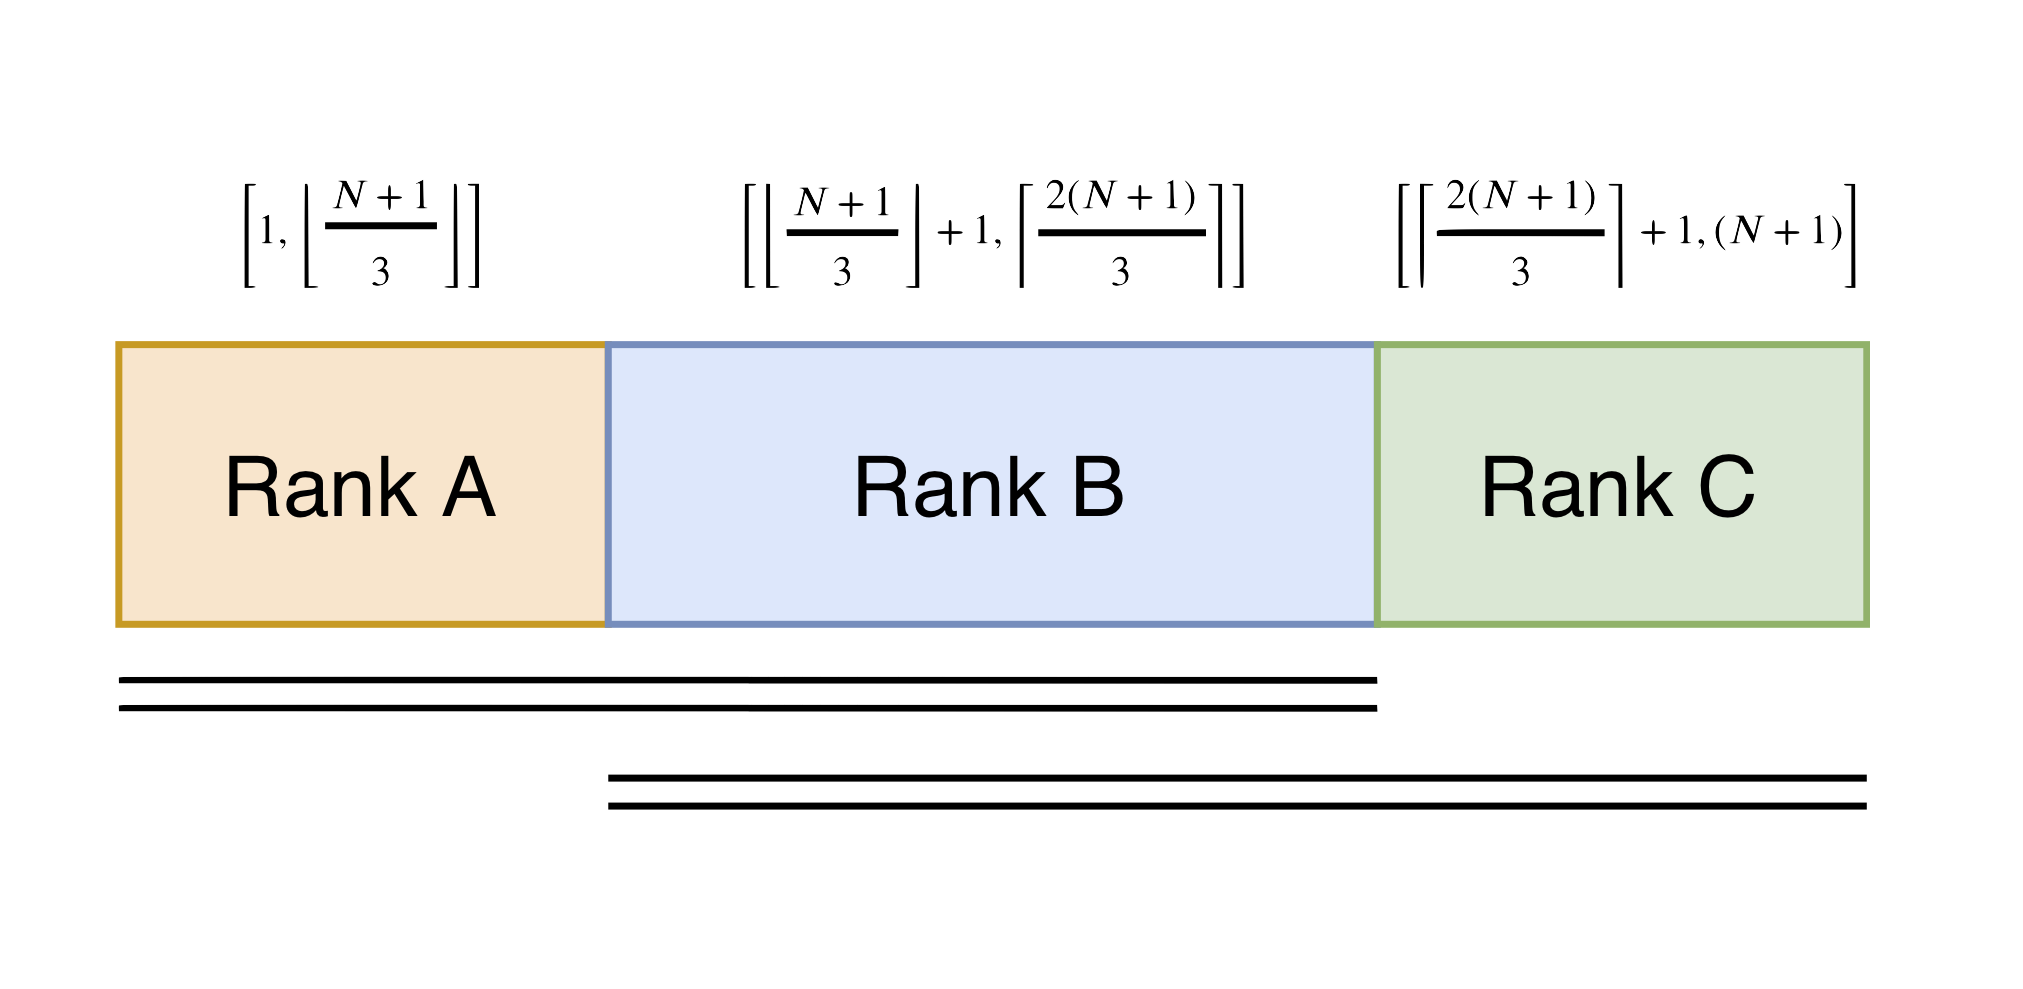
\includegraphics[width=0.75\textwidth]{StoogeFigures/NotPower3.png}
    \caption{Sectors for List Length $\ne 3^k$}
    \textbf{Note:} Underlined segments represent \enquote{two-thirds} elements, $P$.
    \label{fig:notpower3}
\end{figure}
\FloatBarrier

\textbf{Step 1:} Initially, we sort the first two-thirds of our unsorted list (using StoogeSort recursively, which by our induction hypothesis will return a sorted list).  Even in the worst case scenario where all elements of eventual Rank C are in the first two-thirds (or worse, just the first third), \textbf{any element which is of Rank C}---i.e., will eventually reside in indices $\left [ \left \lceil \frac{2(N+1)}{3} \right \rceil +1, (N+1) \right]$---\textbf{and is not already in Rank C indices} must and will be sorted into indices $\left [ \left \lceil \frac{2(N+1)}{3} \right \rceil - \left \lfloor \frac{N+1}{3} \right \rfloor, (N+1) \right]$ (now within the upper two-thirds).  This is because there are $\left \lfloor \frac{N+1}{3}  \right \rfloor$ elements of Rank C, and in the worst case scenario where they all exist in the range $\left [ 1, \left \lceil \frac{2(N+1)}{3} \right \rceil \right ]$ (i.e., within the eventual regions of Rank A and B), by definition and assumption (via our induction hypothesis), these elements of eventual Rank C must be larger (given that they are of Rank C) than anything else in the range of $\left [ 1, \left \lceil \frac{2(N+1)}{3} \right \rceil \right ]$, and so the remnants fill the lowest positions, while these larger $\left \lfloor \frac{N+1}{3}  \right \rfloor$ elements move to the uppermost positions of the first selected two-thirds segment.  See figures \ref{fig:unsorted} and \ref{fig:sort1}. \\

\textbf{Step 2:} Once more recursively using StoogeSort (allowable given our induction hypothesis), we now sort the upper two-thirds of our list (i.e., step 2 of StoogeSort).  Even in the worst case scenario where all elements of eventual Rank A are in the upper two-thirds, \textbf{any} element which is of Rank A---i.e., will eventually reside in indices $\left [ 1, \left \lceil \frac{N+1}{3} \right \rceil \right ]$---\textbf{and not already in the range of Rank A} will be sorted into index range $\left [\left \lfloor \frac{N+1}{3}  \right \rfloor +1, 2 \cdot \left \lfloor \frac{N+1}{3}  \right \rfloor +1\right]$ (now \textit{within the lower two-thirds}).  Like the last step, by definition of Rank A elements (the smallest elements), there may at most be $\left \lfloor \frac{N+1}{3}  \right \rfloor$ Rank A elements which are smaller than any other in the list, so if they all exist in the upper two-thirds, they \textbf{must} move to the lowest indices of the upper two-thirds, assuming StoogeSort works correctly for smaller lists, while the larger remnants fill the upper indices of the upper two-thirds currently being sorted. \\

A similar line of thought follows for any elements of eventual Rank B.  If any existed in this upper two-thirds (again taking two-thirds as defined above in Section \ref{two-thirds}), there are at most $\left \lceil \frac{2(N+1)}{3} \right \rceil - \left \lfloor \frac{N+1}{3}  \right \rfloor$ elements of Rank B in this upper two-thirds, and they must be smaller than all of the elements of eventual Rank C all $\left \lfloor \frac{N+1}{3}  \right \rfloor$ of which now \textbf{must be} in indices $\left [ \left \lceil \frac{2(N+1)}{3} \right \rceil +1, (N+1) \right]$, i.e., their correct indices, given that in the first step \textbf{all} Rank C elements ensured to now be within the upper two-thirds segment (using our induction hypothesis assumes correctness of StoogeSort for smaller list), so the elements of Rank B now must \textbf{all} exist within indices $\left[1, \left \lceil \frac{2(N+1)}{3} \right \rceil \right]$.\\

(\textit{Note: this allows eventual Rank B elements to remain in the index range of Rank A for now given any Rank A elements existed in Rank C index range from the start of the sort and thereby have only now had the opportunity to shift to the lowest range of the two-thirds currently being sorted.}) \\

\textbf{Step 3:} Finally, we sort the first two-thirds again.  At this point, all elements of Rank C are sorted in Rank C's respective indices $\left [ \left \lceil \frac{2(N+1)}{3} \right \rceil +1, (N+1) \right]$.  So all that remain in the first two-thirds are elements of eventual Rank A and Rank B.  Now we are dealing with a sub-list of length < N, so we can assume StoogeSort calls recursively sorts this list correctly; thereby, we are left with a fully sorted list.\\

\rule{\textwidth}{0.4pt}

\textbf{Because StoogeSort works correctly for list of length $N+1$, it is proved by induction that StoogeSort is a correct algorithm.}

\rule{\textwidth}{0.4pt}

%%%%%%%%%%%%%%%%%%%%
%  Stooge RUNTIME  %
%%%%%%%%%%%%%%%%%%%%

\subsection{Recurrence and Run-time}
Given the nature by which StoogeSort recursively calls itself (3 times per list each with sub-list length $P_i$ as defined above where $P_i = \left\lceil\frac{2}{3}\cdot N_i\right\rceil$. \\ 

\rule{\textwidth}{0.4pt}

Translated, then:
$$T(n) = 3T\left(\left\lceil\frac{2}{3}\cdot N\right\rceil \right)$$

Using Master Theorem where $a = 3$, $b = \frac{3}{2}$, $k = 0$ $\implies a > b^k$ we can estimate asymptotic bounds: \\
$$\sim O(n^{log_{\frac{3}{2}}(3)}) \approx O(n^{2.7})$$

\rule{\textwidth}{0.4pt}












%%%%%%%%%%%%%%%%%%
%   Question #2  %
%%%%%%%%%%%%%%%%%%
\newpage

\section{Solving Recurrences}

%%%%%%%%%%%%%%%%%%%%
%   Question #2A   %
%%%%%%%%%%%%%%%%%%%%

\subsection{Part A}
\subsubsection{$T(n)=T(n-1)+4n-4$}
We find (by guess and check and triangular number adding) the exact solution: \\
\rule{\textwidth}{0.4pt}
$$T(n) = 4 \cdot \frac{n(n-1)}{2}+1 = \mathbf{2n(n-1)+1}$$
\rule{\textwidth}{0.4pt}
\textbf{Proving by induction}: \\

Let's show a base case (given $T(1) = 1$).  Using the given recurrence form, $T(2) = T(2-1) + 4(2) - 4 = 5$.  Using our found exact solution, $T(2) = 2(2)(2-1) + 1 = 5$.  Now, suppose (induction hypothesis) our exact solution holds true $\forall n \leq N$.  We hope to show that our solution is true for $N+1$.

\begin{equation}
    T(N+1) = T((N+1) - 1) + 4(N+1) - 4 \? 2(N+1)((N+1)-1) + 1
\end{equation}
Simplified:
\begin{equation} \label{Eqn1SUBSTEP}
    T(N) + 4N \? 2N^2 + 2N + 1
\end{equation}
Now, via our induction hypothesis,  $N \leq N$, we can use our exact solution on the LHS of the equation above (\ref{Eqn1SUBSTEP}).
\begin{equation}
    2N(N-1)+1 + 4N \? 2N^2 + 2N + 1
\end{equation}
Simplified:
\begin{equation}
    2N^2 + 2N + 1 = 2N^2 + 2N + 1
\end{equation}

Our exact solution holds for N+1, so by induction we hold it is true $\forall n$. \\





\subsubsection{$T(n)=2T(n-1)+2n-1$}
We find (by guess and check and loop unrolling) the exact solution: \\
\rule{\textwidth}{0.4pt}
$$T(n) = 2(2^{n}+2^{(n-1)}-(n+1))-1 = \mathbf{3(2^{n}-1)-2n}$$
\rule{\textwidth}{0.4pt}
Proving by induction:
Let's show a base case (given $T(1) = 1$).  Using the given recurrence form, $T(2) = 2T(2-1)+2(2)-1 = 5$.  Using our found exact solution, $T(2) = 3(2^{2}-1)-2(2) = 5$.  Now, suppose (induction hypothesis) our exact solution holds true $\forall n \leq N$.  We hope to show that our solution is true for $N+1$.

\begin{equation}
    T(N+1) = 2T((N+1)-1)+2(N+1)-1 \? 3(2^{N+1}-1)-2(N+1)
\end{equation}
Simplified:
\begin{equation} \label{Eqn2SUBSTEP}
    2T(N) + 2N + 1 \? 6^{N}-2N-5
\end{equation}
Now, via our induction hypothesis,  $N \leq N$, we can use our exact solution on the LHS of the equation above (\ref{Eqn2SUBSTEP}).
\begin{equation}
    2(3(2^{N}-1)-2N) + 2N + 1 \? 6^{N}-2N-5
\end{equation}
Simplified:
\begin{equation}
    6^{N}-2N-5 = 6^{N}-2N-5
\end{equation}

Our exact solution holds for N+1, so by induction we hold it is true $\forall n$. \\




%%%%%%%%%%%%%%%%%%%%
%   Question #2B   %
%%%%%%%%%%%%%%%%%%%%

\subsection{Part B}

\subsubsection{$T(n) = 4T(n/2)+n^3$}
Using Master Theorem to approximate asymptotic bounds, take $a = 4$, $b = 2$, $k = 3$, so $a < b^k$: \\
$$O(n^3)$$

\subsubsection{$T(n) = 17T(n/4)+n^2$}
Using Master Theorem to approximate asymptotic bounds, take $a = 17$, $b = 4$, $k = 2$, so $a > b^k$: \\
$$O(n^{log_{4}(17)}) \sim O(n^{2})$$

\subsubsection{$T(n) = 9T(n/3)+n^2$}
Using Master Theorem to approximate asymptotic bounds, take $a = 9$, $b = 3$, $k = 2$, so $a = b^k$: \\
$$O(n^{2}log(n))$$

\subsubsection{$T(n)=T(\sqrt{n})+1$}
Let's substitute $2^{2^k}$ for $n$. Let $j = log(n) = 2^k$.  We can rewrite our recurrence then: $T(j) = T(\frac{j}{2}) + 1$.  Now using Master Theorem, take $a = 1$, $b = 2$, $k = 0$, so $a = b^k$: \\
$$O(log(j)) = \mathbf{O(log(log(n)))}$$




%%%%%%%%%%%%%%%%%%%
%   Question #3   %
%%%%%%%%%%%%%%%%%%%
\newpage
\section{Longest Path in DAG}

\subsection{Setup}
To efficiently find the longest path in a directed acyclic graph (DAG), we begin by using DFS (as shown in class and section) to topologically sort our DAG (see Lecture 4 notes [p.7]).  After sorting topologically, we must visit all of the edges coming out of nodes in the topological order to begin our calculations of \textit{longest} path.

\subsection{Nodal Analysis}
Initially, we'll set all nodes to have a parent pointer attribute of NIL and path distance attribute of 0 (this path distance indicates the longest path distance which terminates at the node).  Sources (i.e., INDEG = 0) will permanently retain the NIL parent pointer and 0 value path distance attribute (by definition).  Now, we are ready to visit (in topological order) all edges coming out of nodes.  As each path is traversed (from source outward), we will sum a few values to update the path distance attribute of the node currently being visited and update the parent pointer in the following manner:

\begin{enumerate}
    \item Again, if the node is a source, it retains path distance = 0 and parent pointer = NIL.
    \item If the node is not a source and its current path distance value is < (parent node path distance + edge weight), update the current node's path distance to (parent node path distance + edge weight) and change the parent pointer to equal the parent connected to the edge whose weight we just added to update path distance.
    \item If the node is not a source and its current path distance value is $\geq$ (parent node path distance + edge weight), make no change.
\end{enumerate}

A few notes: the method above does handle negative weights insofar as if weights are negative to the extent that they cumulatively sum to a value < 0, unvisited nodes (post-topological sort) will appear to be sources if not considering INDEG (i.e., from a purely path distance and parent pointer perspective) because their path distance will \textbf{remain} 0 rather than changing to the sum of the parent distance + negative edge weight.  If all edge weights in the graph are negative, the algorithm explained above will suggest just remaining at a node as the \enquote{longest} path. \\

Let's explore what this might look like in pseudocode:

\begin{algorithm}
	\caption{Find longest path in a directed acyclic graph (given a topological sort)}
    \label{alg:longpath}
	\begin{algorithmic}
		\For {node $\in$ TOPOLOGICAL SORT}
		\State PathDist $\coloneq 0$
		\State Parent $\coloneq$ NIL
		\EndFor
		
		\For {node $\in$ TOPOLOGICAL SORT} \Comment{for each node in topologically sorted list}
    		\For {(node, v) $\in$ EDGES}\Comment{for each outgoing edge of current node}
        		\If {v.PathDist < [node.PathDist + (node, v).EdgeWeight]}
            		\State v.PathDist $\coloneq$ [node.PathDist + (node, v).EdgeWeight]
            		\State v.Parent $\coloneq$ node
        		\EndIf
        	\EndFor

		\EndFor
		
		\State EndNode $\coloneq$ Max(TOPOLOGICAL SORT$\to$node.PathDist) \Comment{find node with maximal path distance value} \\
		\Comment{if tie, default to first found}
		\State StartNode $\coloneq$ EndNode
		\While {StartNode.Parent != NIL}
		    \State StartNode $\coloneq$ StartNode.Parent
		\EndWhile\\
		\\
		\Return StartNode, EndNode
	\end{algorithmic} 
\end{algorithm} 

\FloatBarrier

\subsection{Proof of correctness}
\subsubsection{Base Case}
Let's show that this \textit{longest path finder} works for a base case of 1 node.  Most importantly, we hope to show correctness for the summing algorithm which assigns each node a value for the longest path distance ending at the node.  In the case of 1 node, it is a standalone source, so after a DFS resulting in topological sort, it is the sole element in the sort.  As it enters the algorithm (see Algorithm \ref{alg:longpath}) the single element is initialized with Path Distance of 0 and Parent pointer of NIL.  Next the algorithm iterates through the topological sort, but since this is a single element graph and the node has no parents (being a source), there is never an opportunity to update its path distance (i.e., remains 0) nor its parent pointer.  This shows, for a 1 element DAG, that the value stored at the node indicating longest path distance ending at the node is correct, as there is no path to/from the source, so its only path is to stay with distance of 0 which is the value reflected by the algorithm.  Now discussing the return procedure of the algorithm (though not the main segment intended to be proved): there are no edges ($\implies$ no children) to explore, so the algorithm enters the final segment to assign EndNode and StartNode which both get assigned to the single node in the Topological Sort because there exist no others, so the maximal path distance is the one of the element (i.e., 0), and the StartNode cannot be reassigned because there are no Parent pointers which are not null.  Returned is the \enquote{longest path} of 0 from the Source, right back to the single element Source.

\subsubsection{Inductive Step}

Suppose Algorithm \ref{alg:longpath} is correct for a number of vertices $n < N$.  Now we hope to show that it will update correctly at node $N+1$ the longest path distance ending at node $N+1$.  For connected elements, assuming DAG, after a topological sort, there exists a few scenarios which might occur when we look to the $(N+1)$th node:
\begin{enumerate}
    \item We see a source.
    \item We see a node with parents (i.e., not a source).
\end{enumerate}

\subsubsubsection{See a source} \label{seeSource}
By definition of a source, the longest path terminating at the source is 0 (as it has no parents $\implies$ no path incoming).  It is easy to show this case, as it models closely our base case.  If node $N+1$ is a source, it will never be updated after the initialization routine, so it will hold its value of longest path distance (ending at the node) of 0 and parent pointer of NIL which matches the definition of a source thereby showing correct operation.  As we move through the rest of the topological sort, its outgoing edge weights will be considered just like all nodes n < N with outgoing edges.  For any child, the outgoing edge weight + $(N+1)$'s stored value (of 0 by definition of source) will be summed and compared, and a future node will update it's parent pointer to $N+1$ if $(N+1)$'s outgoing path is the longest one terminating at the future node.

\subsubsubsection{See a $\mathbf{(N+1)}$th node with parents (i.e., not a source)} \label{seeNotSource}
Given our induction hypothesis, we assume that Algorithm \ref{alg:longpath} is correct for a number of vertices $n < N$; therefore, all of the parents of node $N+1$ have correct values for the longest path distances terminating at each respective parent.  We now might suspect that node $N+1$ will \textbf{not} have updated its path distance value correctly after the algorithm runs.  During the algorithm (while scrolling through the topological sort), if the first parent's path distance + edge weight to the $N+1$ node (negative or not) > $N+1$ path distance (currently 0), node $N+1$ will update it's longest path distance ending at $N+1$ and update its parent pointer to the first parent.  It will continue compare/replacement scheme until all paths from parents to $N+1$ are exhausted in the topological sort.  In the case where every edge weight to $N+1$ had a negative weight of magnitude sufficiently large that [parent's path distance + edge weight to the $N+1$ node] < 0 for every each iteration, the $N+1$ node would not ever update its longest path distance terminating at itself ($N+1$) indicator, and its parent pointer would remain NIL.  This thereby ensures that, in fact, our algorithm \textit{will} update correctly and store at node $N+1$ the longest path distance terminating at node $N+1$. As we move through the rest of the topological sort, $(N+1)$'s outgoing edge weights will be considered just like all nodes n < N with outgoing edges.  For any child, the outgoing edge weight + $(N+1)$'s stored value (of 0 by definition of source) will be summed and \textit{compared}, and a future node will update it's parent pointer to $N+1$ if $(N+1)$'s path distance value + outgoing edge weight results in the longest path terminating at the future node. \\

In either scenario (\ref{seeSource}, \ref{seeNotSource}), since the longest path terminating at each node and the parent pointer corresponding to that longest path is stored correctly for all nodes, the final segment of our Algorithm \ref{alg:longpath} will always return the correct StartNode and EndNode.  \textit{Hooray!}

\subsection{Runtime}
\subsubsection{Setup}
The initial topological sort runs in $O(|V| + |E|)$.

\subsubsection{Maximal Distance Search}
The dual loop only touches every edge once, iterating through the parent nodes (summing edge weights) leads to the \enquote{meat} of our algorithm running in $O(|V| + |E|)$ time.

\subsubsection{Re-trace Longest Path}
Finally, at worst, when finding the StartNode and Endnode, we might touch every edge and every node once at worst, leading to--once more---$O(|V| + |E|)$ time
$\implies$ \textbf{total runtime:} $\mathbf{O(|V| + |E|)}$







%%%%%%%%%%%%%%%%%%%
%   Question #4   %
%%%%%%%%%%%%%%%%%%%
\newpage
\section{Buffy's Nighttime Patrol}

\subsection{Setup/Assumptions}
We will assume that Sunnydale is a city where all intersections are connected (i.e., a single connected component).

For Buffy's slaying technique, suppose Sunnydale's intersections are nodes on an undirected graph, and its streets are edges on the graph.  I suggest the following augmentation to a depth-first search of a connected \textbf{undirected} graph:

\begin{enumerate}
    \item Starting at any vertex (i.e., any intersection), begin the depth first search and keep track of (1) visited vertices and (2) visited edges [\textbf{note}: undirected graph, so (u,v) $\in$ E is synonymous with (v,u) $\in$ E].
    \item Unlike a typical DFS, \textbf{if a vertex} (i.e., any intersection) connected via an edge (i.e., a street) to the current vertex \textbf{has been visited}, check to see if the edge has been traversed.  If the edge hasn't been traveled, but the vertex \textbf{has} been visited, traverse the edge and immediately return (i.e., go down the street and come right back).  Do \textbf{not}, however, travel down an untraveled edge to an already visited vertex if there exist other unvisited vertices to visit (with edges from current node available to reach these unvisited vertices).  Visit the unvisited, connected vertices first.
    \item If both the next connected vertex and shared edge have been visited and traversed, respectively, do not interact with the pair.
\end{enumerate}

For all intents and purposes, as the augmented DFS (made specially for Sunnydale) progresses, Buffy could visually keep track of the stack.  As items are pushed onto the stack, Buffy would walk toward those vertices from her current node.  As items are popped off the stack, Buffy would know to return to the highest remaining element on the stack.  \textbf{One caveat} is that in our augmented DFS, we need to push onto the stack those vertices which we visit despite their already being visited (i.e., vertex has been visited but edge hasn't been traversed, so we traverse and immediately return) and pop those vertices.

\subsection{Proof}
\subsubsection{Base Cases}
Let's walk through how the Slaying algorithm might operate for a city with one street (i.e., two nodes and 1 edge).  After topological sort, Buffy would start at the first intersection (vertex) listed and traverse the street (edge) in one direction to the unvisited intersection (vertex).  At this next intersection, given our instructions, Buffy would see no further vertices or edges to explore, and would return to the start intersection [traveling in the other direction, i.e., the other side of the street] (by seeing the stack pop off the intersection/vertex at which she currently stands). \\

Let's take a tougher base case of three intersections (vertices) with two streets (edges) and then three intersections with three streets.  \textit{(It is worth noting the loose usage of the term intersection which can mean just a dead-end to a street, not always the confluence of two or more streets.)}  

\subsubsubsection{Base Case: 3 intersections with 2 streets} In the case of two streets, three intersections (picture a linear setup), let's suppose Buffy will start at the leftmost intersection/vertex (because this offers a more complex case than starting at the center intersection).  Buffy traverses the street to the middle intersection/vertex in one direction because it hasn't been explored.  Now at the middle intersection, Buffy \textbf{must} explore the rightmost intersection because our algorithm (augmented DFS) requires her to explore unvisited vertices/intersections \textbf{before} returning to the intersection from where she came.  This shows that Buffy will not inhibit travel to the rightmost intersection (and subsequently on the rightmost street) by backtracking too soon and taking a bi-directional street (all streets in Sunnydale are bi-directional) out of play.  So Buffy goes to explore the rightmost intersection and there sees nowhere else to travel and therefore returns home, in the other direction, successfully traversing each side of all streets only once.

\subsubsubsection{Base Case: 3 intersections with 3 streets} 
In the case of 3 streets, three intersections (picture a triangular setup with vertices \{A,B,C\}), let's suppose Buffy will start any intersection/vertex, A.  Buffy traverses any one of the two connected streets to a vertex (we'll say B) in one direction because it hasn't been explored.  Now at the intersection B, Buffy \textbf{must} explore intersection C because our algorithm (augmented DFS) requires her to explore unvisited vertices/intersections \textbf{before} returning to the intersection from where she came.  So Buffy goes to explore the intersection C and there sees no unexplored vertices but does see an additional unexplored street/edge (back to intersection A).  By our algorithm's rules, Buffy goes to intersection A (this is her second time there because she started her slay patrol there) and comes right back (to C) (thereby traversing both sides of the previously last remaining untraveled street/edge).  Seeing no fully un-traversed streets nor unvisited intersections, Buffy simply returns to her start (A), thereby, traversing all sides of all streets.  \textbf{BUT}, what prevents Buffy, at A from going to C?  We've marked the A$\to$C street/edge as visited, so in our augmented DFS, that street is not re-traveled.

\subsubsection{Semi-Inductive Step}
Suppose we take a Sunnydale layout in undirected graph representation where intersections (and dead-ends) are nodes and streets are undirected edges.  Let's assume that our method has worked to direct Buffy, seeing nodes $n \leq N-1$, thus far (i.e., no excessive street traversals).  Given our algorithm's specification and the requirement that we have a \textbf{connected} graph, the $N$th node \textbf{must} be explored at some point before Buffy returns to the start by operation of a correct DFS and our stipulations (if there exists an unvisited node and an edge leading to it, it must be explored before any return trips to visited nodes).  If the $N$th node stands alone (single connection), Buffy will turn back after visiting; else, the exploration continues, yet eventually (by DFS and our stipulations of return if both all connected nodes + edges have been visited) will return to the $N-1$th node from where Buffy came.  The same induction may be taken on edges, rather than nodes, as even in the scenario where all edges ($N$, v) at a node, $N$, lead to already explored other vertices, our algorithm enforces that an edge (if un-traveled) to an explored vertex must be traveled in a \enquote{go and come back} method.  So at this point, it is preserved that Buffy only travels each street in each direction once.





%%%%%%%%%%%%%%%%%%%
%   Question #5   %
%%%%%%%%%%%%%%%%%%%
\newpage
\section{Heaps!}
\subsection{Merge K-Sorted Lists w/ N Total Elements}
\subsubsection{Process}
A divide-and-conquer method (while seemingly obvious) doesn't use heaps (or at least binary heaps), so we needed a way to exploit the pre-sorted nature of each list.  Our suggestion is to use a single binary heap in the following way (supposing lists sorted max-first):

\begin{enumerate}
    \item From the k-presorted lists, select the max from each (i.e., PeekMax, which is O(1) as discussed in Section, k times) and build a binary heap (BuildHeap, which is O(k) time---for k elements---as discussed in section).
    \item With each element in the binary heap, store an indicator value that shows from which of the k-sorted lists the element on the heap originated, e.g., (VALUE, Origin List).
    \item From the now built heap, \textbf{remove} the max element (the root) via ExtractMax which runs in O(log(k)) time (as shown in section notes) and \textbf{replace} the removed element with the next largest element (i.e., just the next element since already sorted) in the list from which it originated (check the aforementioned indicator while removing)---the replacement (via Insert) takes O(log(k)) time (as shown in section notes).
    \item If no list items remain on the list from which the just extracted element originated, then proceed without replacement (noting that the ExtractMax operation retains a balanced binary heap).
    \item This process (excluding the one-time build heap) iterates until $\exists$ no more elements on any list nor the heap (i.e., it can repeat an upper-bound n times).
\end{enumerate}

\subsubsection{Runtime}
As mentioned in the steps above, the merge algorithm involves a one-time build-heap cost of O(k) plus an ExtractMax and Insert cost of O(log(k)) + O(log(k)) n times:

$$O(n \cdot 2log(k))$$ 
which, in essence, is 
$$O(nlog(k))$$

\subsubsection{Proof}
\subsubsubsection{Base Case}
Let us show that for $k$-lists of $n$-total elements, the first element is selected and sorted correctly.  Suppose the lists are sorted \{max, min\}.  We select the first element from each of $k$-lists, which means---by reason of the $k$-lists being internally sorted---we must have on hand the maximal element of the entire set of n elements.  BuildHeap creates a max binary heap which then contains the selected first elements from the $k$-lists, thereby placing the maximal element of the entire set at the root of the heap.  ExtractMax then removes this maximal element placing it in our destination fully sorted, merged list.  So, our method works to sort the first of $n$ total elements.

\subsubsubsection{Inductive Step}
Let us assume that our algorithm sorts correctly for all elements n $\leq$ $N-1$.  Now we hope to show that our algorithm sorts correctly the Nth element.  We know by the requirements of our algorithm, that it contains the maximal remaining element from each of $k$-lists (so long as one exists, i.e., the list has not been fully cleared) and that the sorted/merged list up to this point $(N-1)$ has removed from our heap and $k$ origin lists \textbf{all} larger elements.  Again, with this known state (i.e., our heap \textbf{must} contain the maximal remaining element from each of k-lists) when ExtractMax, then, is called on our max binary heap, the next largest element exists in our heap, so it is correctly removed given the correct operation of ExtractMax (shown in Section notes) and placed on our merged/sorted list $\therefore$ our algorithm operates correctly for the $N$th element.



\subsection{Sort List of K-Close to Sorted List}
\subsubsection{Process}
Let's assume a list which prioritizes max elements (though this is quite the same implementation for a min-list):
\begin{enumerate}
    \item Build a binary heap (one time cost) of the first k elements.
    \item ExtractMax from this binary heap and Insert the next element from the k-close-to-sorted list.
    \item If no element remains on the k-close-to-sorted list, proceed without Insert.
    \item This process (excluding the one-time build heap) iterates until $\exists$ no more elements on the list nor nodes on the heap.
\end{enumerate}

\subsubsection{Runtime}
As mentioned in the steps above, the sorting algorithm involves a one-time build-heap cost of O(k) plus an ExtractMax and Insert cost of O(log(k)) + O(log(k)) n times:

$$O(n \cdot 2log(k))$$ 
which, in essence, is 
$$O(nlog(k))$$

\subsubsection{Proof}
\subsubsubsection{Base Case}
Suppose we have a list $k$-close to sorted \{max, min\}.  We hope to show that using our algorithm, the first element will be selected and sorted correctly.  We know that in a $k$-close to sorted list indexed [0, $n$] (I apologize from switching from 1-indexing in Problem \#1 to 0-indexing now), the maximal element will at most be in the range of indices [0, $k-1$].  Since we select $k$ elements to add to our max binary heap in its initial build, we include all elements from our $k$-close to sorted list within indices [0, $k-1$].  Thereby, our heap \textbf{must} contain the maximal element of our unsorted list.  ExtractMax is performed on our heap and then must remove the root element which was the largest in the initial $k$-close to sorted list, placing it in a fully sorted list.  Thereby, our method works to find the first element.

\subsubsubsection{Inductive Step}
Let us assume that our algorithm sorts correctly for all elements $n$ $\leq$ $N-1$.  Now we hope to show that our algorithm sorts correctly the $N$th element.  We know---given the definition of $k$-close to sorted---that the $N$th element of our sorted list exists in the original list within indices [$N-(k-1)$, $N+(k-1)$], and at this step given our inductive hypothesis and correct prior operation of the algorithm for $n$ $\leq$ $N-1$, all elements [0, $N+(k-1)$] have existed on the heap and have been extracted and placed in our sorted list \textbf{or} exist \textit{now} on the max binary heap, thereby containing the next largest element.  ExtractMax is performed on our heap and then must remove the root element which is the largest outstanding element, placing it in the $N$th position of the fully sorted list.  Thereby, our method works to find the $N$th element. 






%%%%%%%%%%%%%%%%%%%
%%%%%%%%%%%%%%%%%%%
%%%%%%%%%%%%%%%%%%%
%    APPENDIX     %
%%%%%%%%%%%%%%%%%%%
%%%%%%%%%%%%%%%%%%%
%%%%%%%%%%%%%%%%%%%
\newpage
\section{APPENDIX} \label{APPENDIX}

\subsection{StoogeSort: Powers of 3 list length}

To prove by induction, and given the correctness of our base case, let us assume (induction hypothesis) that StoogeSort is correct for all lists of size $n \leq N$.  We seek to show that StoogeSort is a correct sorting algorithm for lists of size $N+1$. Let's first take the case where the number of elements, $N+1$,  in the list is a power of 3 (i.e., we can express $N+1 = 3^k = 3j$ for integers $j, k$).  Next, since the list can be divided by three all the way down (i.e., recursively) to the base case where a list entered recursively into StoogeSort is of length 3 (\enquote{two-thirds sublist} = length of 2), and because we assume that StoogeSort is correct $\forall n \leq N$, we can assume that any recursive call to StoogeSort on a sub-list will result in a sorted list output.  We can assign \enquote{ranks} or \enquote{sector labels} to each third of the list such that when sorted, the list elements in the first third (i.e., the lowest) will be of Rank A, list elements of the top third (i.e., the highest value) will be of Rank C, and the third in the middle will be of Rank B when the list is sorted (see Figure \ref{fig:ranks}).  More formally, Rank A spans indices $[1, j]$, Rank B spans [j+1, 2j], and Rank C spans [2j+1, 3j] or [2j+1, N+1].

\begin{figure}[h]
    \centering
    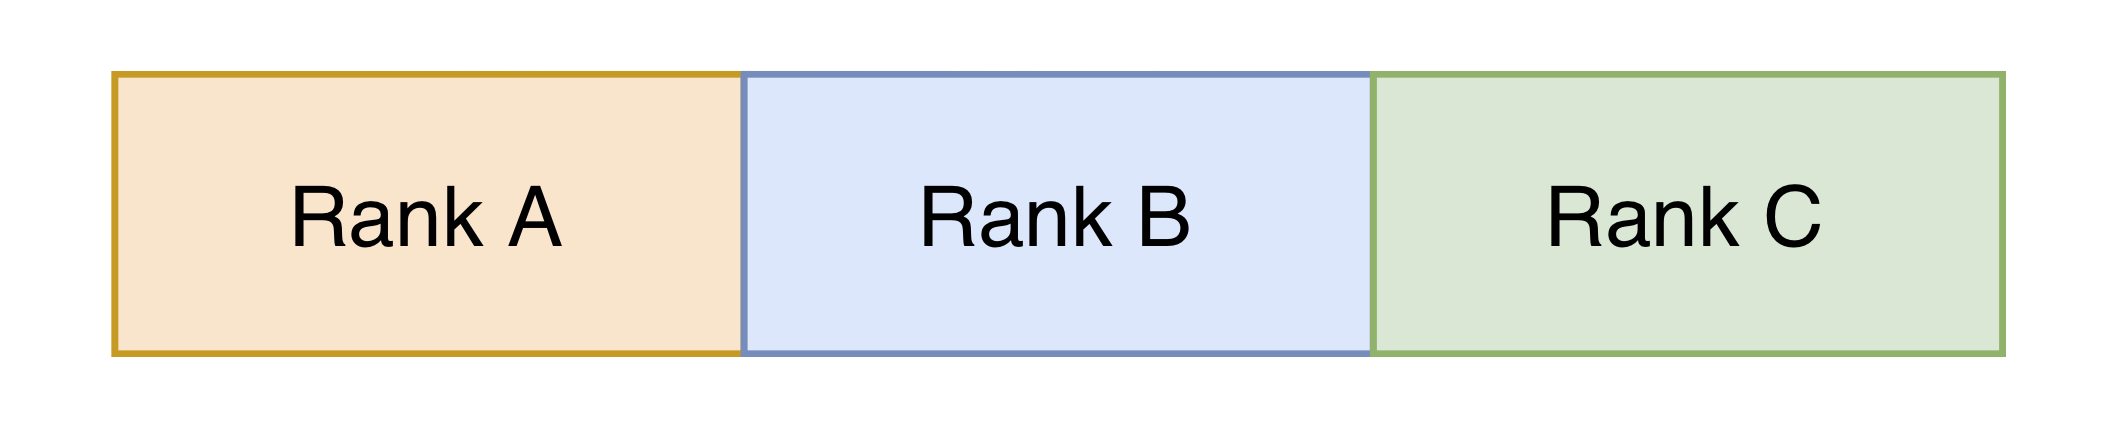
\includegraphics[width=0.75\textwidth]{StoogeFigures/Rank.png}
    \caption{Ranked by Thirds}
    \label{fig:ranks}
\end{figure}
\FloatBarrier

Initially, we sort the first two-thirds of our unsorted list (using StoogeSort recursively, which by our induction hypothesis will return a sorted list).  Even in the worst case scenario where all elements of eventual Rank C are in the first two-thirds (or worse, just the first third), any element which is of Rank C (i.e., will eventually reside in indices [2j+1, N+1]) and is not already in Rank C indices must and will be sorted into indices [j+1, 2j] (the lower-third of the upper two-thirds).  This is because there can at most be j elements of Rank C, and in the worst case scenario where they all exist in the range [1, 2j] (i.e., within the eventual regions of Rank A and B), by definition and assumption (via our induction hypothesis), these j elements of eventual Rank C must be larger (given that they are of Rank C) than anything else in the range of [1,2j], and so the remnants fill the lowest third [1,j] and these largest j elements move to the middle third [j+1, 2j].  See figures \ref{fig:unsorted} and \ref{fig:sort1}.

\begin{figure}[h]
    \centering
    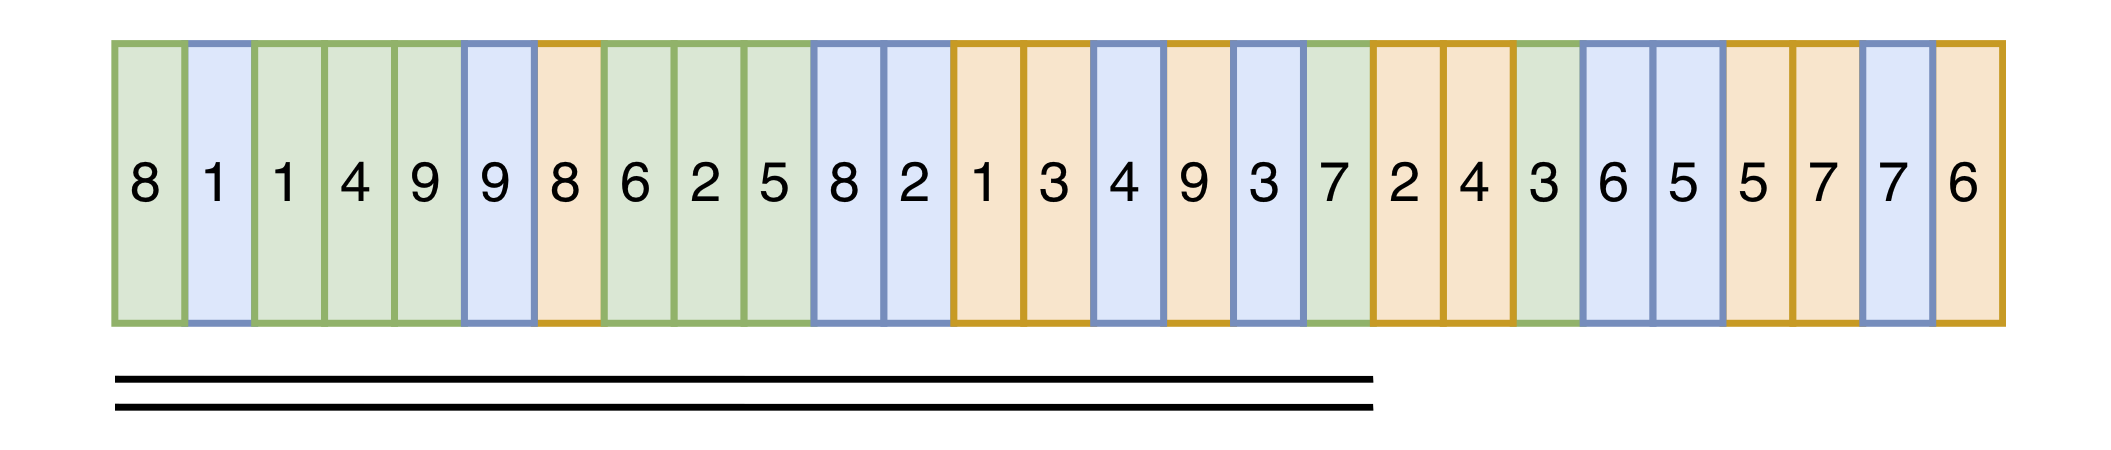
\includegraphics[width=0.75\textwidth]{StoogeFigures/Unsorted.png}
    \caption{Unsorted (List of 27 (i.e., power of 3)) [portion \textbf{underlined} to be sorted]}
    \label{fig:unsorted}
\end{figure}
\FloatBarrier

\begin{figure}[h]
    \centering
    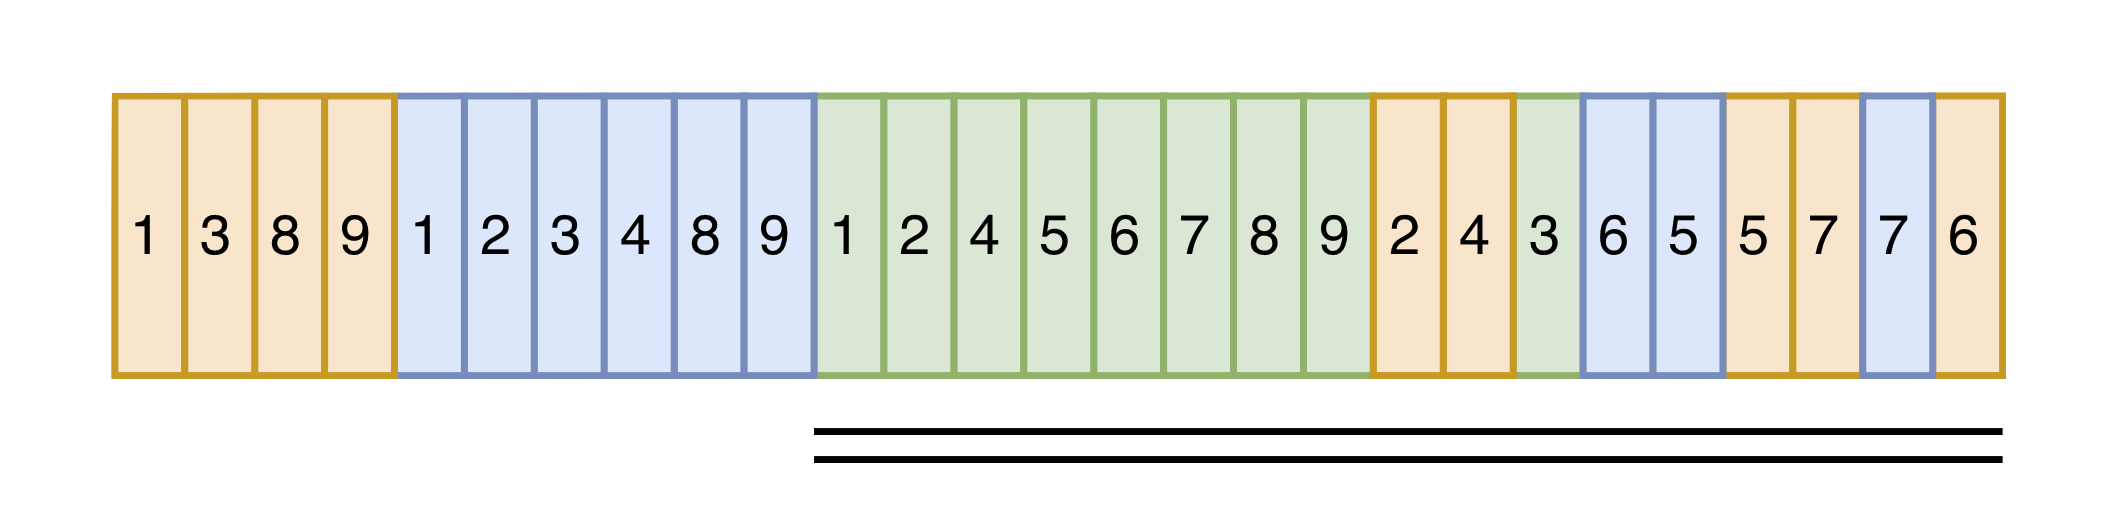
\includegraphics[width=0.75\textwidth]{StoogeFigures/Sort1.png}
    \caption{First two-thirds sorted (any element of eventual Rank C now in upper two-thirds)}
    \label{fig:sort1}
\end{figure}
\FloatBarrier

Once more recursively using StoogeSort (allowable given our induction hypothesis), we sort the upper two-thirds of our list.  Even in the worst case scenario where all elements of eventual Rank A are in the upper two-thirds, any element which is of Rank A (i.e., will eventually reside in indices [1, j]) and not already in [1,j] will be sorted into index range [j+1, 2j] (in the pictured scenario---see figure \ref{fig:sort2}---some elements of Rank A resided in Rank A at the start, so now after the second sort, all elements of Rank A reside within indices [1, 2j]).  Like the last step, by definition of Rank A elements (the lowest third), there may at most be $j$ Rank A elements which are smaller than any other in the list, so if they all exist in the upper two-thirds, they must move to indices [j+1, 2j] while the larger remnants fill the uppermost third. \\
\\
A similar line of thought follows for any elements of eventual Rank B.  If any existed in indices [j+1, N+1], there are at most $j$ elements of Rank B in this upper two-thirds, and they must be smaller than all of the elements of eventual Rank C all $j$ of which are in indices [j+1, N+1], so the elements of Rank B now must \textbf{all} exist in indices [1, 2j]. \\

Similarly in the prior stated worst case scenario where all elements of eventual Rank C were in the first two-thirds but sorted into indices [j+1, 2j] during the first sorting step, these Rank C elements (and thereby \textbf{all} Rank C elements) are now sorted correctly, residing at their final destination indices [2j+1, N+1], again because there are $j$ Rank C elements, and since they're larger than all other elements in the list and already reside in [j+1, N+1], they must take the uppermost third [2j+1, N+1] leaving the remnants to the middle-third [j+1, 2j].  See figure \ref{fig:sort2}.

\begin{figure}[h]
    \centering
    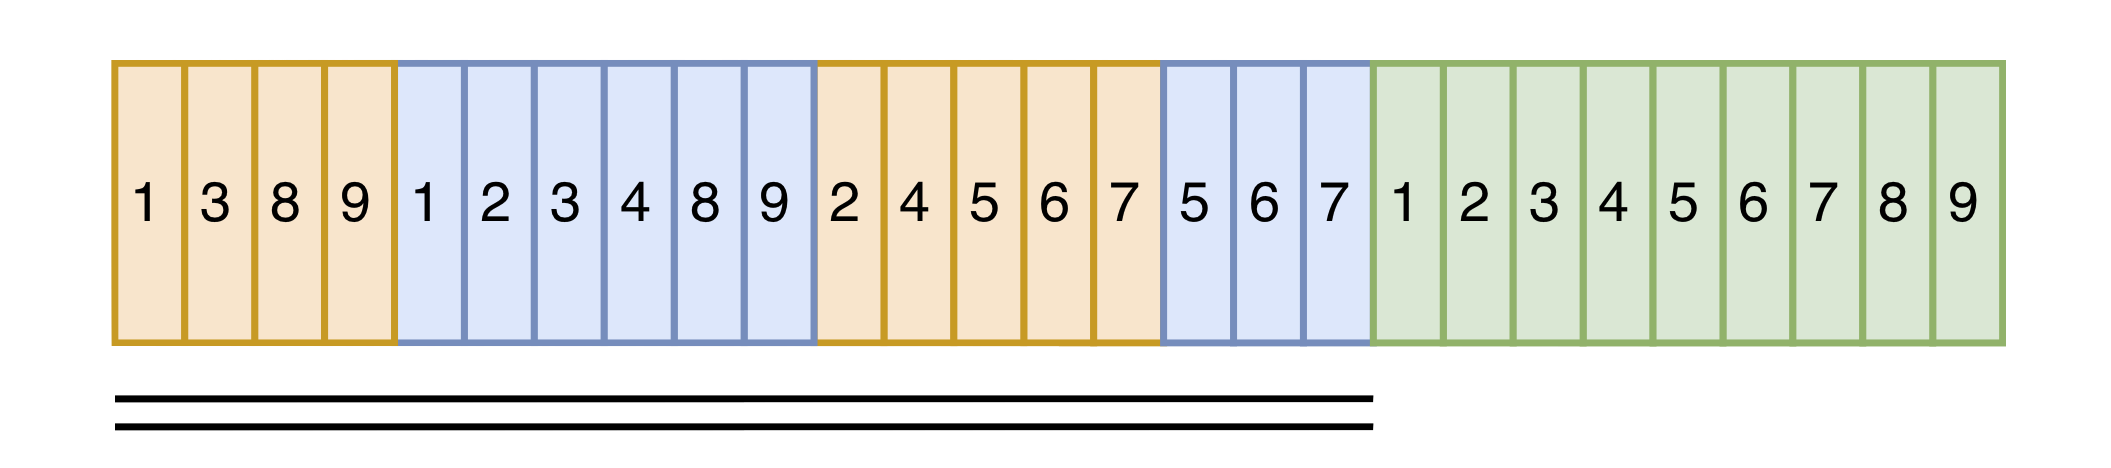
\includegraphics[width=0.75\textwidth]{StoogeFigures/Sort2.png}
    \caption{Upper two-thirds sorted (any element of eventual Rank C now fully sorted in indices [2j+1, $N+1$])}
    \textit{(any element of eventual Rank A exists within indices [1, 2j])}
    \label{fig:sort2}
\end{figure}
\FloatBarrier

Finally, we sort the first two-thirds again.  At this point, all elements of Rank C are sorted in Rank C's respective indices [2j+1, N+1].  So all that remain in the first two-thirds are elements of eventual Rank A and Rank B.  Now we are dealing with a sub-list of length < N, so we can assume StoogeSort calls recursively sorts this list correctly; thereby, we are left with a fully sorted list. See figure \ref{fig:sorted}.

\begin{figure}[h]
    \centering
    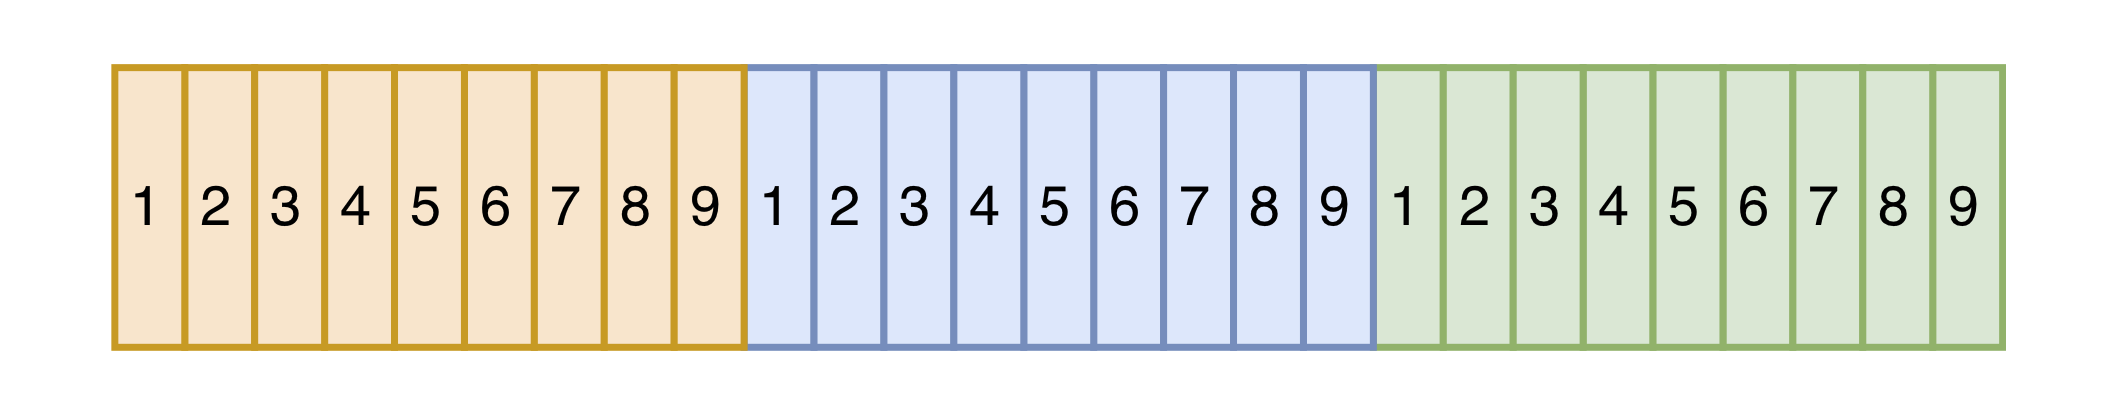
\includegraphics[width=0.75\textwidth]{StoogeFigures/Sorted.png}
    \caption{First two-thirds re-sorted $\implies$ fully sorted list}
    \label{fig:sorted}
\end{figure}
\FloatBarrier

\end{document}
